% ============================================================
%  Cap{\'i}tulo IV  -  Experimentaci{\'o}n y Resultados
%  (Se inserta entre Metodolog{\'i}a (III) y Factibilidad, que pasa a V.)
%  Secci{\'o}n 4.1: Caracterizaci{\'o}n y preparaci{\'o}n del corpus (EDA).
%  Integra TODO el informe EDA del curso (7 figuras + tablas) en formato APA 7
%  (encabezados, tablas/figuras con n{\'u}mero y t{\'i}tulo arriba y Nota al pie).
%  Figuras: imagenes/eda_*.png (copiadas del EDA del curso).
% ============================================================
\section{Experimentaci\'on y Resultados}
\label{cap:experimentacion}

Este cap{\'i}tulo presenta la evidencia emp{\'i}rica obtenida al ejecutar la metodolog{\'i}a
del Cap{\'i}tulo~III. Se inicia con la caracterizaci{\'o}n y preparaci{\'o}n del corpus,
pues la validez de toda m{\'e}trica posterior depende de la calidad y de la partici{\'o}n
de los datos con que se entrena y eval{\'u}a el sistema. El an{\'a}lisis exploratorio de
datos (EDA) precede al modelamiento para que cada decisi{\'o}n se tome sobre evidencia
num{\'e}rica y no sobre supuestos \parencite{hernandez2018metodologia}.

\subsection{Caracterizaci\'on y preparaci\'on del corpus (EDA)}
\label{sec:eda}

El m{\'o}dulo de reconocimiento de voz (ASR) de esta tesis se construye sobre el
subconjunto \texttt{validated} de Common Voice 27.0, variedad quechua sure{\~n}o
(\texttt{qxp}). Al igual que otros corpus de voz en lenguas originarias, es un recurso
valioso pero escaso y con sesgos de recolecci{\'o}n que deben documentarse antes de usarlo
\parencite{zevallos2022huqariq}. El punto de partida fueron \textbf{22\,727} clips
validados; cada clip aporta su audio, su transcripci{\'o}n y metadatos del hablante. Se
aplic{\'o} un protocolo de an{\'a}lisis exploratorio de cinco pasos ---primer vistazo,
calidad, anatom{\'i}a num{\'e}rica, correlaciones y variable objetivo--- cuyo detalle
reproducible (\emph{scripts} y \emph{notebook}) se incluye en los Anexos.

\subsubsection{El dataset y las variables de an\'alisis}
\label{sec:eda-variables}

A las columnas originales del corpus se a{\~n}aden variables derivadas de la \emph{forma del
habla}, {\'u}tiles para diagnosticar el audio y su transcripci{\'o}n
(Tabla~\ref{tab:eda-variables}).

\begin{table}[H]
  \centering
  \caption{Variables de an\'alisis del corpus \texttt{qxp}}
  \label{tab:eda-variables}
  \small
  \begin{tabularx}{\linewidth}{@{}l l X@{}}
    \toprule
    Variable & Tipo & Significado \\
    \midrule
    \texttt{dur\_s} & num\'erica & Duraci\'on del audio en segundos. \\
    \texttt{n\_chars}, \texttt{n\_words} & num\'erica & Longitud de la transcripci\'on (caracteres / palabras). \\
    \texttt{cps} & num\'erica & Velocidad de habla $=$ \texttt{n\_chars}/\texttt{dur\_s} (car/s). \\
    \texttt{up\_votes}, \texttt{down\_votes}, \texttt{net\_votes} & num\'erica & Votos de validaci\'on comunitaria. \\
    \texttt{sentence\_domain} & categ\'orica & Dominio tem\'atico (multi-etiqueta). \\
    \texttt{age}, \texttt{gender}, \texttt{accents} & categ\'orica & Metadatos demogr\'aficos del hablante. \\
    \texttt{client\_id} & categ\'orica & Identificador del hablante (77 en total). \\
    \bottomrule
  \end{tabularx}
  \notaAPA{Las variables \texttt{dur\_s}, \texttt{n\_chars}, \texttt{n\_words} y \texttt{cps}
  son derivadas. Elaboraci{\'o}n propia a partir de Common Voice 27.0.}
\end{table}

El primer vistazo (\texttt{describe}) sit{\'u}a la duraci{\'o}n media en \textbf{4,83\,s}
(rango 1,8--14,9), las frases entre 11 y 83 caracteres y la velocidad media en
\textbf{7,27\,car/s}. Dos columnas (\texttt{variant} y \texttt{segment}) aparecen
completamente vac{\'i}as desde el inicio.

\subsubsection{Calidad y limpieza de los datos}
\label{sec:eda-calidad}

\textbf{Valores faltantes.} La Figura~\ref{fig:eda-nulos} mapea los nulos: \texttt{variant}
y \texttt{segment} son 100\,\% nulas; \texttt{accents}, 63,2\,\%; y \texttt{gender},
27,9\,\%. Por tratarse de metadatos demogr{\'a}ficos que \emph{no invalidan} el audio ni su
transcripci{\'o}n, se marcan como \texttt{unknown} en vez de borrar filas: eliminar por
\texttt{accents} costar{\'i}a casi dos tercios del corpus.

\begin{figure}[H]
  \centering
  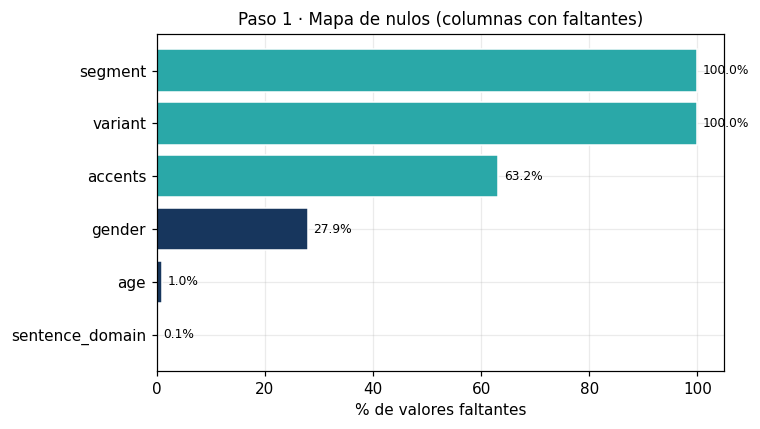
\includegraphics[width=0.72\linewidth]{eda_fig1_nulos.png}
  \caption{Porcentaje de valores faltantes por columna}
  \label{fig:eda-nulos}
  \notaAPA{En turquesa, las columnas inservibles ($\ge$50\,\% de nulos). Elaboraci{\'o}n
  propia.}
\end{figure}

\textbf{Duplicados y fuga potencial.} No hay filas ni audios repetidos, pero solo existen
\textbf{2\,067 frases {\'u}nicas}: cada una se grab{\'o} $\approx$11 veces por distintos
hablantes. No es un defecto ---es lo esperable en un corpus ASR multi-hablante---, pero
obliga a \textbf{particionar por frase o por hablante} para evitar \emph{fuga de datos}
(Secci{\'o}n~\ref{sec:eda-particion}). \textbf{Errores.} La etiqueta \texttt{sentence\_domain}
es multi-valor; 76 filas repiten \emph{tokens} internos y se corrigen deduplicando. Ning{\'u}n
clip validado tiene \texttt{net\_votes}\,$\le$\,0.

\subsubsection{Anatom\'ia num\'erica y desbalances}
\label{sec:eda-anatomia}

El histograma y el diagrama de caja leen los mismos datos de forma distinta: el primero
muestra la \emph{forma} de la distribuci{\'o}n; el segundo, la mediana, la dispersi{\'o}n y
los valores at{\'i}picos (Figuras~\ref{fig:eda-hist} y~\ref{fig:eda-box}). Las
distribuciones son unimodales, con leve asimetr{\'i}a a la derecha, y exhiben colas que
exponen clips extremos en duraci{\'o}n y velocidad.

\begin{figure}[H]
  \centering
  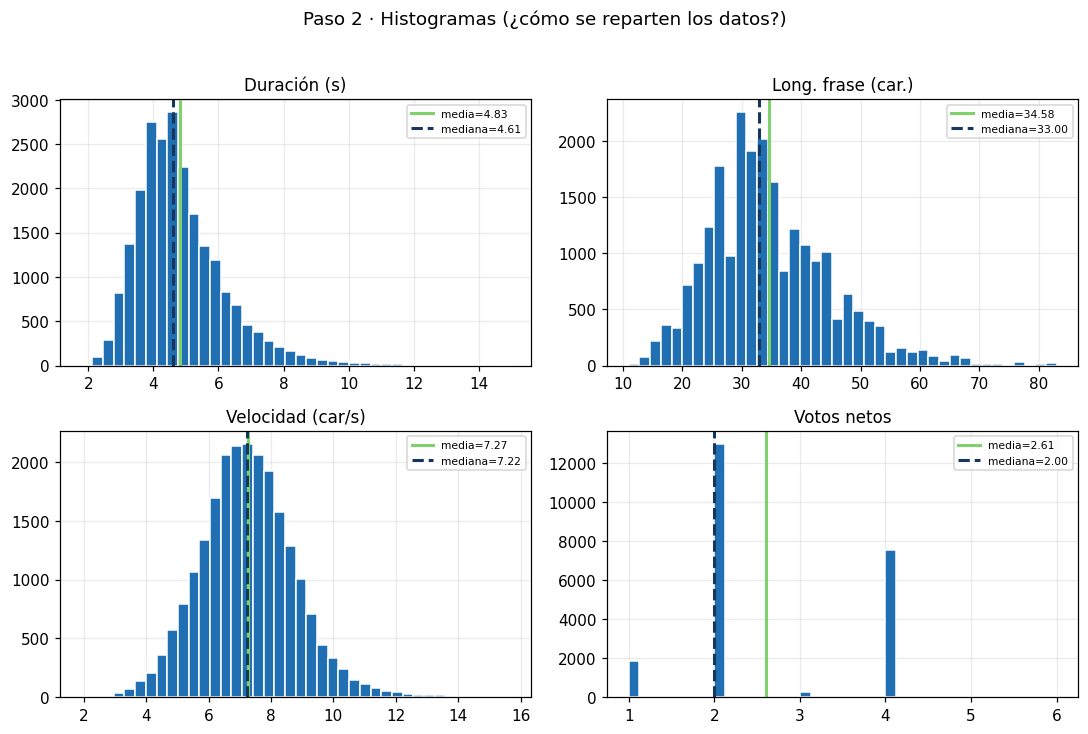
\includegraphics[width=0.82\linewidth]{eda_fig2_histogramas.png}
  \caption{Histogramas de las variables num\'ericas}
  \label{fig:eda-hist}
  \notaAPA{Distribuciones unimodales con leve asimetr{\'i}a a la derecha. Elaboraci{\'o}n
  propia.}
\end{figure}

\begin{figure}[H]
  \centering
  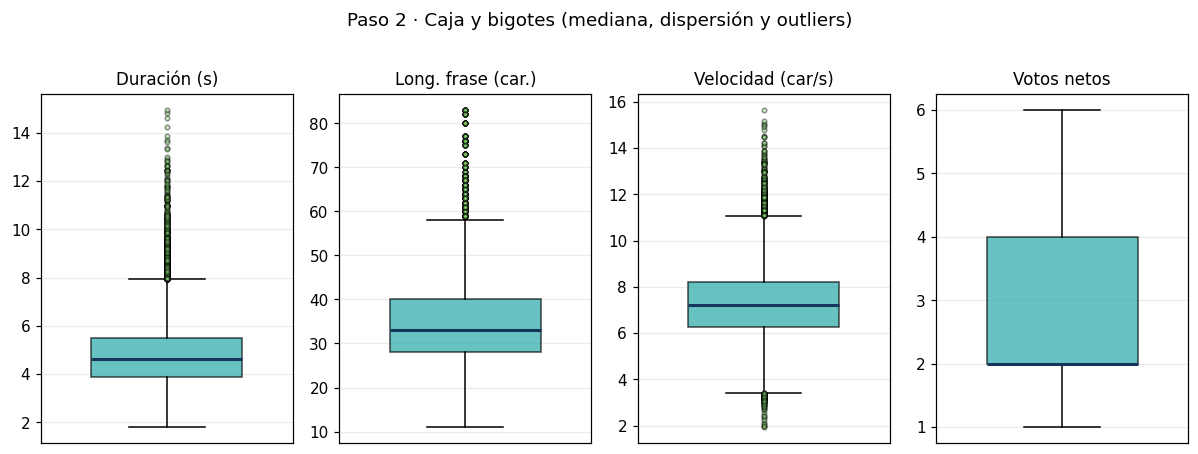
\includegraphics[width=\linewidth]{eda_fig3_boxplots.png}
  \caption{Diagramas de caja y bigotes de las variables num\'ericas}
  \label{fig:eda-box}
  \notaAPA{Las colas de puntos exponen clips extremos de duraci{\'o}n y velocidad
  (desajuste audio--texto). Elaboraci{\'o}n propia.}
\end{figure}

El an{\'a}lisis de las variables categ{\'o}ricas (Figura~\ref{fig:eda-barras}) revela los
hallazgos m{\'a}s importantes del diagn{\'o}stico:

\begin{itemize}\itemsep1pt
  \item \textbf{G{\'e}nero severamente desbalanceado}: 16\,079 \texttt{female} frente a
        solo \textbf{308} \texttt{male} (y 6\,340 \texttt{unknown}). Un modelo entrenado
        as{\'i} aprender{\'a} sobre todo voz femenina: sesgo que debe declararse como
        limitaci{\'o}n para un uso m{\'e}dico con pacientes de ambos sexos.
  \item \textbf{Edad} concentrada en \texttt{twenties} y \texttt{thirties}.
  \item \textbf{Dominio salud}: $\approx$\textbf{78\,\%} de los clips incluyen
        \texttt{healthcare}, cobertura favorable para la tesis m{\'e}dica.
  \item \textbf{Concentraci{\'o}n de hablantes}: un {\'u}nico hablante aporta
        \textbf{8,9\,\%} del corpus (2\,013 clips), lo que refuerza la partici{\'o}n por
        hablante.
\end{itemize}

\begin{figure}[H]
  \centering
  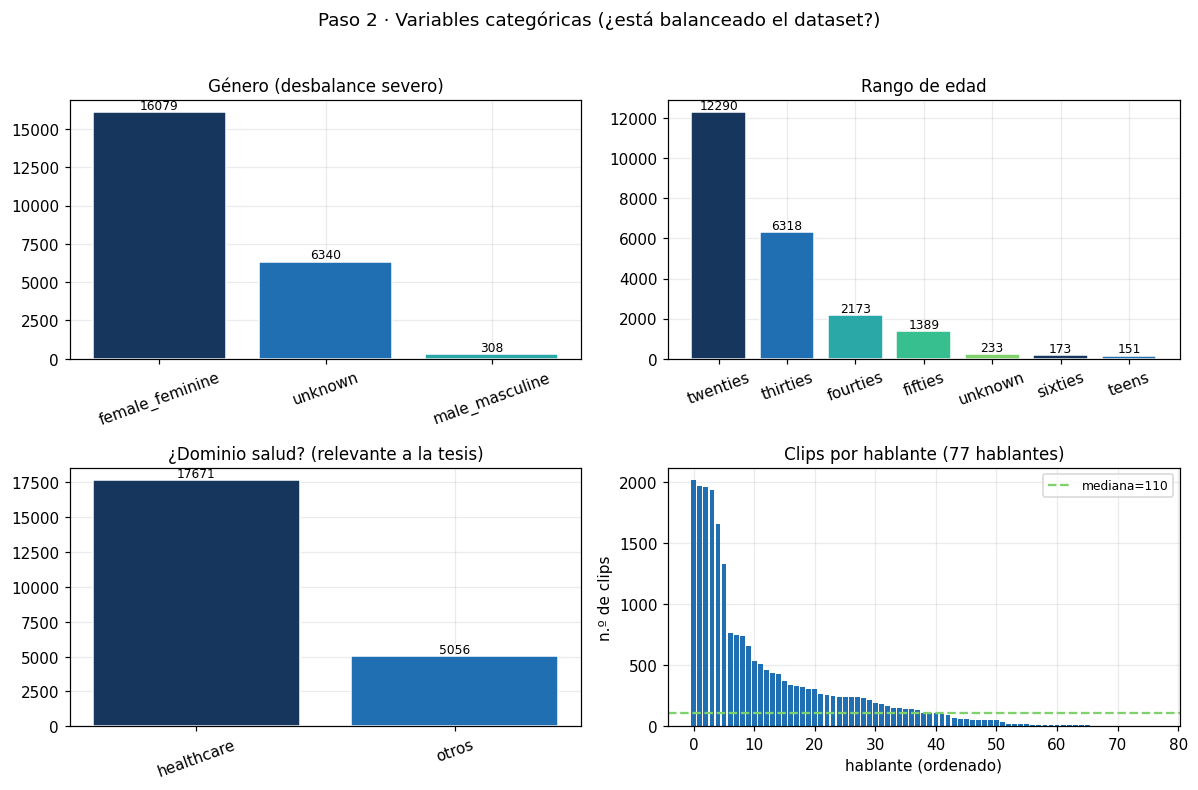
\includegraphics[width=\linewidth]{eda_fig4_barras.png}
  \caption{Distribuci\'on de las variables categ\'oricas del corpus}
  \label{fig:eda-barras}
  \notaAPA{El g{\'e}nero y la concentraci{\'o}n de hablantes son los desbalances
  cr{\'i}ticos. Elaboraci{\'o}n propia.}
\end{figure}

\subsubsection{Correlaciones: Pearson y Spearman}
\label{sec:eda-correlaciones}

La longitud de la frase y la duraci{\'o}n del audio se mueven juntas en diagonal ascendente
(Figura~\ref{fig:eda-disp}): relaci{\'o}n positiva y lineal. La velocidad frente a la
duraci{\'o}n es d{\'e}bilmente negativa, por un efecto de borde en clips muy cortos.

\begin{figure}[H]
  \centering
  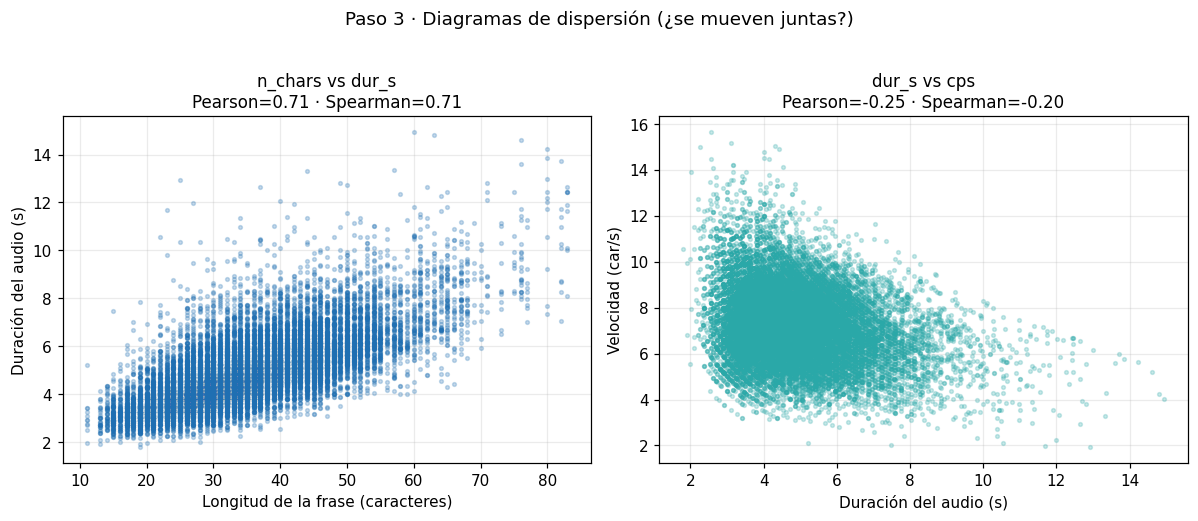
\includegraphics[width=\linewidth]{eda_fig5_dispersion.png}
  \caption{Diagramas de dispersi\'on con sus coeficientes de Pearson y Spearman}
  \label{fig:eda-disp}
  \notaAPA{Elaboraci{\'o}n propia.}
\end{figure}

Se reportan ambos coeficientes (Figura~\ref{fig:eda-heat}): \textbf{Pearson} mide la
asociaci{\'o}n \emph{lineal}; \textbf{Spearman}, basado en rangos, mide la \emph{monoton{\'i}a}
y es robusto a valores at{\'i}picos y a la no-normalidad. Coinciden en relaciones limpias
(\texttt{dur\_s}\,$\sim$\,\texttt{n\_chars}\,$=0{,}71$) pero divergen donde hay asimetr{\'i}a:
\texttt{down\_votes}\,$\sim$\,\texttt{net\_votes} vale $-0{,}37$ (Pearson) frente a $-0{,}50$
(Spearman). Esa diferencia justifica usar ambas m{\'e}tricas y no fiarse de una sola.

\begin{figure}[H]
  \centering
  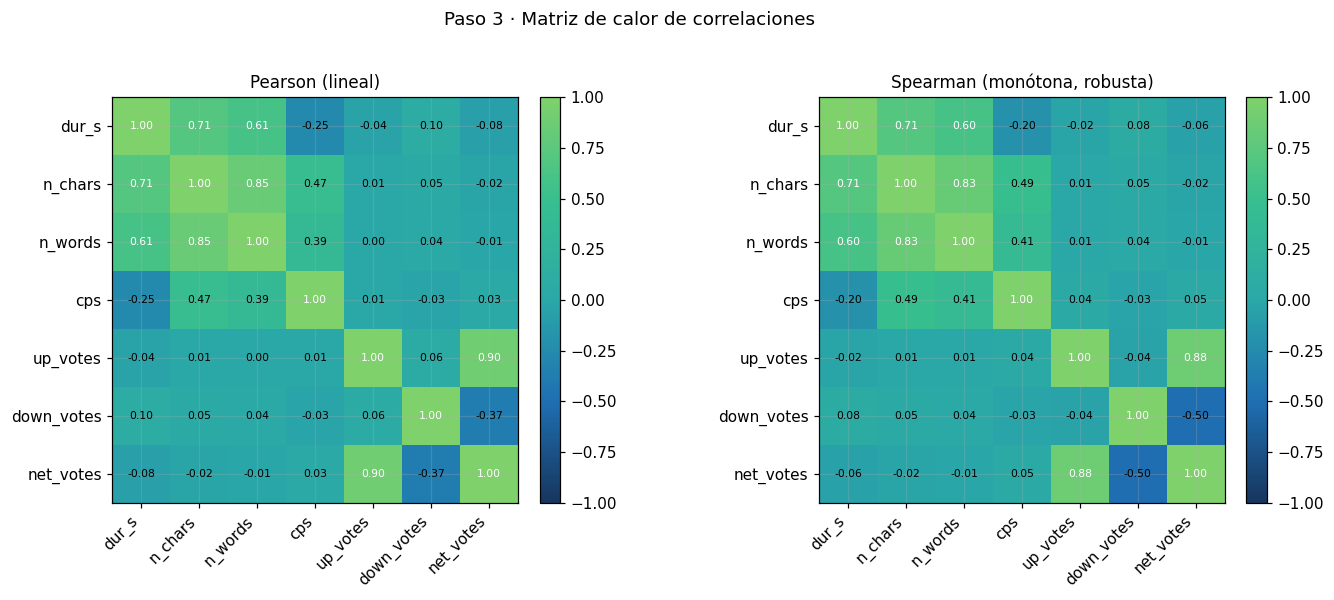
\includegraphics[width=\linewidth]{eda_fig6_heatmaps.png}
  \caption{Matrices de calor de correlaci\'on de Pearson y de Spearman}
  \label{fig:eda-heat}
  \notaAPA{Izquierda: Pearson (lineal). Derecha: Spearman (mon{\'o}tona, robusta).
  Elaboraci{\'o}n propia.}
\end{figure}

\subsubsection{Variable objetivo: dominio de salud}
\label{sec:eda-salud}

Como la investigaci{\'o}n se orienta a la consulta m{\'e}dica, se cruzaron las variables de
forma por el indicador \texttt{is\_healthcare} (Figura~\ref{fig:eda-obj}). El subconjunto de
salud muestra frases algo m{\'a}s cortas (mediana 32 frente a 36 caracteres) y ligeramente
m{\'a}s lentas. Las diferencias son peque{\~n}as pero \textbf{estad{\'i}sticamente
significativas} (prueba de Mann--Whitney, $p \ll 0{,}001$) por el gran tama{\~n}o muestral.
El dominio cl{\'i}nico, que cubre el \textbf{77,8\,\%} del corpus limpio, est{\'a} bien
representado y es homog{\'e}neo con el resto, sin sesgos de forma que dificulten el ajuste.

\begin{figure}[H]
  \centering
  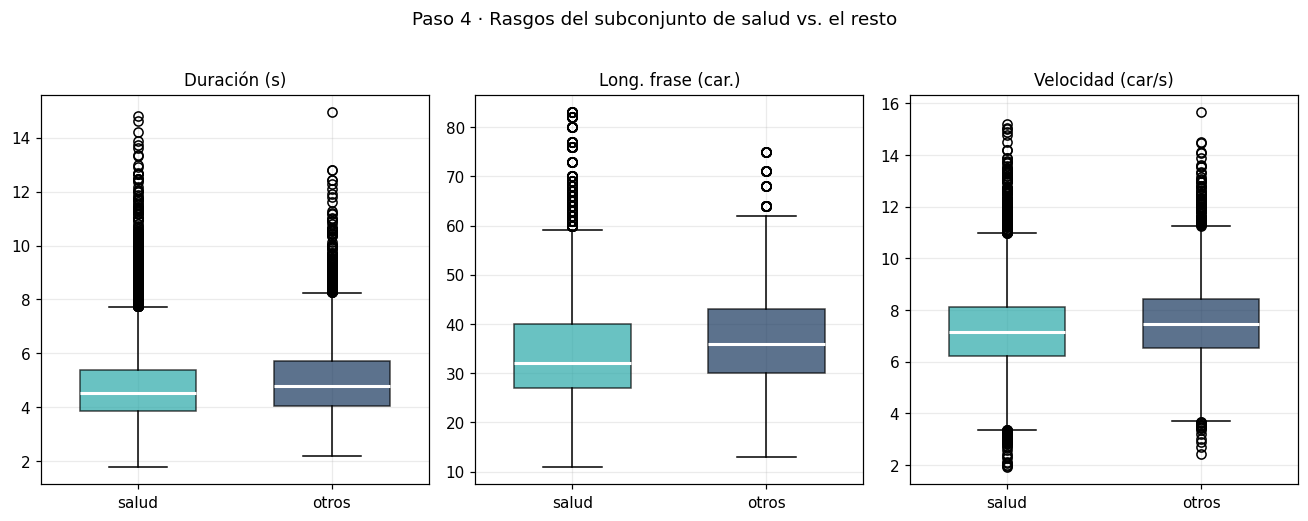
\includegraphics[width=\linewidth]{eda_fig7_objetivo.png}
  \caption{Gr\'aficos cruzados: subconjunto de salud frente al resto del corpus}
  \label{fig:eda-obj}
  \notaAPA{Elaboraci{\'o}n propia.}
\end{figure}

\subsubsection{Dataset limpio resultante}
\label{sec:eda-limpieza}

Respetando el orden del protocolo ---primero limpiar, luego una variable, luego dos y al
final el objetivo--- se obtiene el dataset depurado. El criterio de inclusi{\'o}n para
entrenamiento es: sin valor at{\'i}pico por la regla intercuart{\'i}lica de Tukey en
\texttt{dur\_s} y \texttt{cps}, y \texttt{net\_votes}\,$>$\,0. El corpus pas{\'o} de
\textbf{22\,727} a \textbf{21\,653} clips (Tabla~\ref{tab:eda-limpieza}).

\begin{table}[H]
  \centering
  \caption{Decisiones de limpieza y su efecto sobre el corpus}
  \label{tab:eda-limpieza}
  \small
  \begin{tabularx}{\linewidth}{@{}X r@{}}
    \toprule
    Decisi\'on de limpieza & Efecto \\
    \midrule
    Eliminar columnas vac\'ias, constantes o redundantes & $-4$ columnas \\
    Normalizar \texttt{sentence\_domain} (deduplicar \emph{tokens}) & 76 filas corregidas \\
    Imputar nulos demogr\'aficos como \texttt{unknown} & 0 filas perdidas \\
    Excluir at\'ipicos (IQR) de duraci\'on y velocidad & $-1\,074$ filas (4,7\,\%) \\
    \midrule
    \textbf{Corpus validado crudo} $\rightarrow$ \textbf{dataset limpio} & \textbf{22\,727 $\rightarrow$ 21\,653} \\
    \bottomrule
  \end{tabularx}
  \notaAPA{La regla intercuart{\'i}lica (criterio de Tukey) se aplic{\'o} sobre
  \texttt{dur\_s} y \texttt{cps}. Elaboraci{\'o}n propia.}
\end{table}

\subsubsection{Normalizaci\'on ortogr\'afica del quechua}
\label{sec:eda-normalizacion}

La tasa de error del ASR es sensible a diferencias ortogr{\'a}ficas invisibles en la
referencia. Se fij{\'o} una convenci{\'o}n {\'u}nica y documentada: forma Unicode NFC;
unificaci{\'o}n de las variantes tipogr{\'a}ficas del ap{\'o}strofo al ap{\'o}strofo recto
\texttt{'} ---preservando su valor \emph{fon{\'e}mico} como marca de glotalizaci{\'o}n en
las oclusivas quechuas (\emph{p', t', ch', k', q'})---; conversi{\'o}n a min{\'u}sculas;
retiro de la puntuaci{\'o}n no pronunciada conservando ap{\'o}strofo y gui{\'o}n internos; y
colapso de espacios. La normalizaci{\'o}n afect{\'o} al \textbf{99,9\,\%} de las
transcripciones y redujo las frases {\'u}nicas del dataset limpio de 2\,062 a \textbf{2\,058}
al fundir variantes equivalentes. No se hallaron d{\'i}gitos en el texto, por lo que no fue
necesario desambiguar n{\'u}meros hablados.

\subsubsection{Partici\'on anti-fuga: el \emph{trade-off} hablante\,/\,frase}
\label{sec:eda-particion}

El re{\'u}so masivo de frases obliga a controlar la \emph{fuga de datos}. Se evaluaron los
dos ejes de partici{\'o}n posibles, cada uno disjunto en un eje y midiendo la fuga residual
en el otro (Tabla~\ref{tab:eda-particion}). El hallazgo es que ambos ejes son
\textbf{incompatibles} en este corpus: como casi todos los hablantes graban las mismas
2\,058 frases, una partici{\'o}n disjunta por hablante deja el $\sim$100\,\% de las frases
de prueba tambi{\'e}n en entrenamiento, y una disjunta por frase deja el $\sim$100\,\% de
las voces compartidas.

\begin{table}[H]
  \centering
  \caption{Las dos particiones (80/10/10 por n\'umero de clips) y su fuga residual}
  \label{tab:eda-particion}
  \small
  \begin{tabularx}{\linewidth}{@{}l r r r X@{}}
    \toprule
    Partici\'on & Train & Val & Test & Fuga residual (test) \\
    \midrule
    Disjunta por \textbf{hablante} & 17\,139 & 2\,260 & 2\,254 & 100\,\% de las \emph{frases} ya vistas \\
    Disjunta por \textbf{frase}    & 17\,309 & 2\,168 & 2\,176 & 100\,\% de las \emph{voces} ya vistas \\
    \bottomrule
  \end{tabularx}
  \notaAPA{Semilla \texttt{SEED=42}. Ambas particiones quedan fijadas en columnas
  reproducibles del dataset (\texttt{split\_sentence}, \texttt{split\_speaker}).
  Elaboraci{\'o}n propia.}
\end{table}

Para un ASR m{\'e}dico, cuyo objetivo es transcribir \emph{frases nuevas} dichas en
consulta mediante un modelo de base tipo Whisper \parencite{radford2023whisper}, la
amenaza m{\'a}s grave es que el modelo memorice el repertorio fijo de frases. Por ello se
adopta la \textbf{partici{\'o}n disjunta por frase} como principal, y se conserva la
disjunta por hablante como evaluaci{\'o}n complementaria de robustez ante voces no vistas;
el solapamiento de hablantes se declara como limitaci{\'o}n.

\subsubsection{S\'intesis, rigor e implicaciones}
\label{sec:eda-sintesis}

El EDA entrega un corpus de 21\,653 clips depurados, con texto normalizado y dos
particiones verificadas sin fuga en su eje respectivo. El estudio se apoya en cuatro
dimensiones de rigor: \emph{metodol{\'o}gica} (orden estricto del protocolo; cada decisi{\'o}n
sobre evidencia num{\'e}rica), \emph{te{\'o}rica} (Pearson y Spearman complementarios, regla
IQR de Tukey, contrastes de Mann--Whitney), \emph{interpretativa} (cada figura con su lectura,
distinguiendo hallazgos reales de asociaciones triviales) y \emph{replicabilidad} (semilla
fija, versiones registradas, resultados deterministas).

De este an{\'a}lisis se derivan tres decisiones que gobiernan el resto del cap{\'i}tulo:
(i) evaluar con la partici{\'o}n disjunta por frase y reportar tambi{\'e}n la disjunta por
hablante; (ii) informar la tasa de error \emph{estratificada por g{\'e}nero} para exponer el
sesgo del desbalance 16\,079\,/\,308; y (iii) usar este corpus depurado ---no el crudo---
como base del factor «calidad del corpus» del experimento de ablaci{\'o}n descrito en la
metodolog{\'i}a (Tabla~\ref{tab:ablacion}). Todo el proceso es reproducible mediante los
\emph{scripts} \texttt{eda\_limpieza.py} y \texttt{particionar\_dataset.py} de los Anexos.

% ------------------------------------------------------------
% Las secciones 4.2 (resultados ASR), 4.3 (resultados MT quy->quz),
% 4.4 (resultados TTS) y 4.5 (an{\'a}lisis de error) se completar{\'a}n al ejecutar
% los experimentos. El experimento de ablaci{\'o}n de calidad de corpus ya est{\'a}
% formalizado en el Cap{\'i}tulo III (Tabla~\ref{tab:ablacion}).
% ------------------------------------------------------------
